% -----------------------------------------------
% Template for ISMIR Papers
% 2015 version, based on previous ISMIR templates
% -----------------------------------------------

\documentclass{article}
\usepackage{ismir,amsmath,cite}
\usepackage{graphicx}
\usepackage{color}
\usepackage{mathrsfs}
\usepackage[english]{babel}
\usepackage{caption}
\usepackage{subfig, color}
\usepackage{microtype}
\usepackage{IEEEtrantools}
\sloppy

\usepackage{xspace}
\newcommand*{\eg}{e.g.\@\xspace}
\newcommand*{\ie}{i.e.\@\xspace}

% Title.
% ------
\title{Learning pitch invariants for instrument recognition}


% Single address
% To use with only one author or several with the same address
% ---------------
\oneauthor
{Names should be omitted for double-blind reviewing}
{Affiliations should be omitted for double-blind reviewing}
%\oneauthor
%{Vincent Lostanlen, Carmine Emanuele Cella, and St\'{e}phane Mallat}
%{\'{E}cole normale sup\'{e}rieure}

% Two addresses
% --------------
%\twoauthors
%  {First author} {School \\ Department}
%  {Second author} {Company \\ Address}

% Three addresses
% --------------
%\threeauthors
 %{First author} {Affiliation1 \\ {\tt author1@ismir.edu}}
 %{Second author} {\bf Retain these fake authors in\\\bf submission to preserve the formatting}
 %{Third author} {Affiliation3 \\ {\tt author3@ismir.edu}}

% Four addresses
% --------------
%\fourauthors
%  {First author} {Affiliation1 \\ {\tt author1@ismir.edu}}
%  {Second author}{Affiliation2 \\ {\tt author2@ismir.edu}}
%  {Third author} {Affiliation3 \\ {\tt author3@ismir.edu}}
%  {Fourth author} {Affiliation4 \\ {\tt author4@ismir.edu}}

\begin{document}
%
\maketitle
%
\begin{abstract}
Musical performance combines a wide range of pitches, nuances, and expressive techniques.
Audio-based classification of musical instruments thus requires to build signal representations that are invariant to such transformations.
Focusing on pitch invariance, this article investigates the construction of multi-stage architectures for instrument recognition.
We show that Mel-frequency cepstral coefficients (MFCC) lack invariance with respect to realistic pitch shifts.
In turn, a convolutional neural network (ConvNet) in the time-frequency domain is able to disentangle pitch variability from timbral information in a subtler way.
We further improve the ConvNet architecture by limiting weight sharing to octave-wide frequency bands at the first layer, while allowing full weight sharing at deeper layers.
We extend our method to the recognition of multiple instruments playing simultaneously.
\end{abstract}
%

\section{Introduction}\label{sec:introduction}
Among the cognitive attributes of musical tones, pitch is distinguished by a combination of three properties.
First, it is relative: ordering pitches from low to high gives rise to intervals and melodic patterns.
Secondly, it is intensive: multiple pitches heard simultaneously produce a chord, not a single unified tone -- contrary to loudness, which adds up with the number of sources.
Thirdly, it is invariant to instrumentation: this makes possible the transcription of polyphonic music under a single symbolic system. 

Section 2 demonstrates that pitch is the major factor of variability among musical notes of a given instrument, if described by their Mel-frequency cepstra.
Section 3 describes a typical deep learning architecture for spectrogram-based classification, consisting of two convolutional layers and one densely connected layer.
Section 4 improves the aforementioned architecture by splitting spectrograms into octave-wide frequency bands, training specific convolutional layers over each band in parallel, and gathering feature maps at a later stage.
Section 5 discusses the effectiveness of the presented systems on a challenging dataset for music instrument recognition.


% The problem is made difficult by the fact that factors of variability are entangled.

% Deep convolutional networks have proven to disentangle factors of variability in computer
% vision, such as pose, color, and lighting conditions.


% the challenge is thus two-fold
% 1. gaining abstraction by integrating time-frequency patterns over longer time scales
% 2. building invariants to melody while remaining highly discriminative to the instrument


% On music instrument classification
% Ref to Joder et al
% Ref to Fuhrmann

% On feature learning
% Ref to Dieleman and Benjamin ICASSP 2014
% Ref to Humphrey, Bello, LeCun 2012
% Ref to Salamon and Bello
% Ref to Li, Qian, and Wang arXiv 2015

\section{How invariant is the Mel cepstrum ?}
The MFCCs were extracted from a filterbank of 40 Mel-frequency bands and 13 discrete cosine transform coefficients.

\begin{figure}[t]
    \begin{center}
        \setlength{\unitlength}{1cm}
        \begin{picture}(8.5,9)
        \put(0.1,0){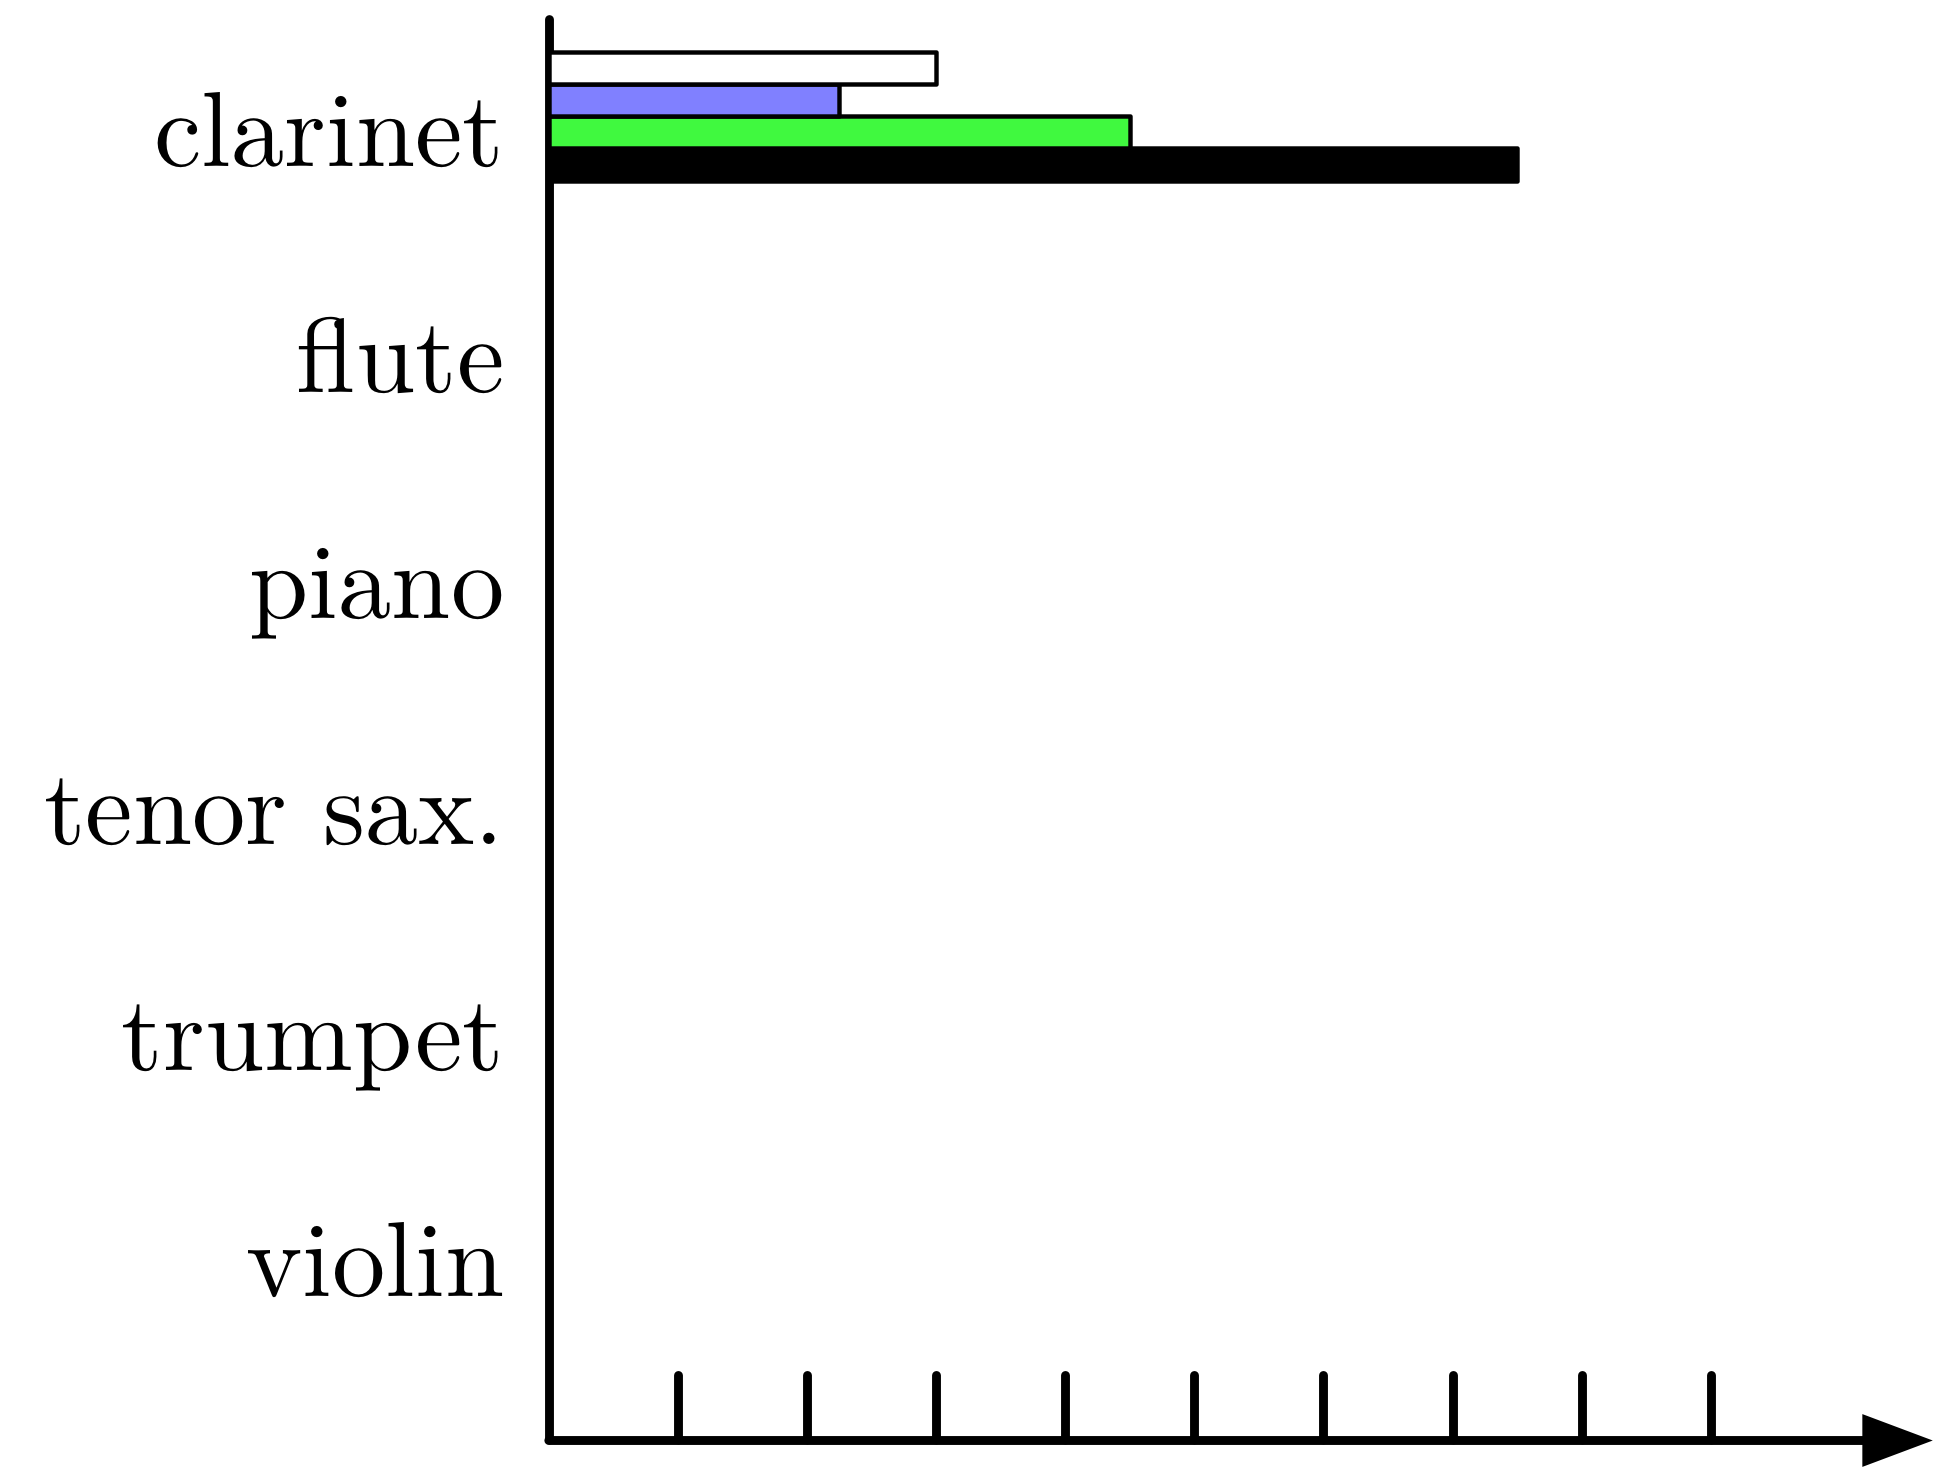
\includegraphics[width=8cm]{figs/mfcc_variances.png}}
        \end{picture}
    \end{center}
    \protect\caption{
Distributions of squared Euclidean distances among various clusters in the RWC dataset. Whisker ends correspond to lower and upper deciles. See text for details.
\label{fig:instrument-distribution}
}
\end{figure}
 
\section{Deep convolutional networks}
A deep learning system for classification is built by stacking multiple layers of weakly nonlinear transformations, whose parameters are jointly optimized such that the top-level layer fits a training set of labeled examples.
This section introduces a typical deep learning architecture for audio classification and describes the functioning of each layer.
% For music instrument classification, this objective function is a histogram of the active instruments within an audio stream.

\begin{figure*}[t]
    \begin{center}
        \setlength{\unitlength}{1cm}
        \begin{picture}(17,5)
        \put(0,0){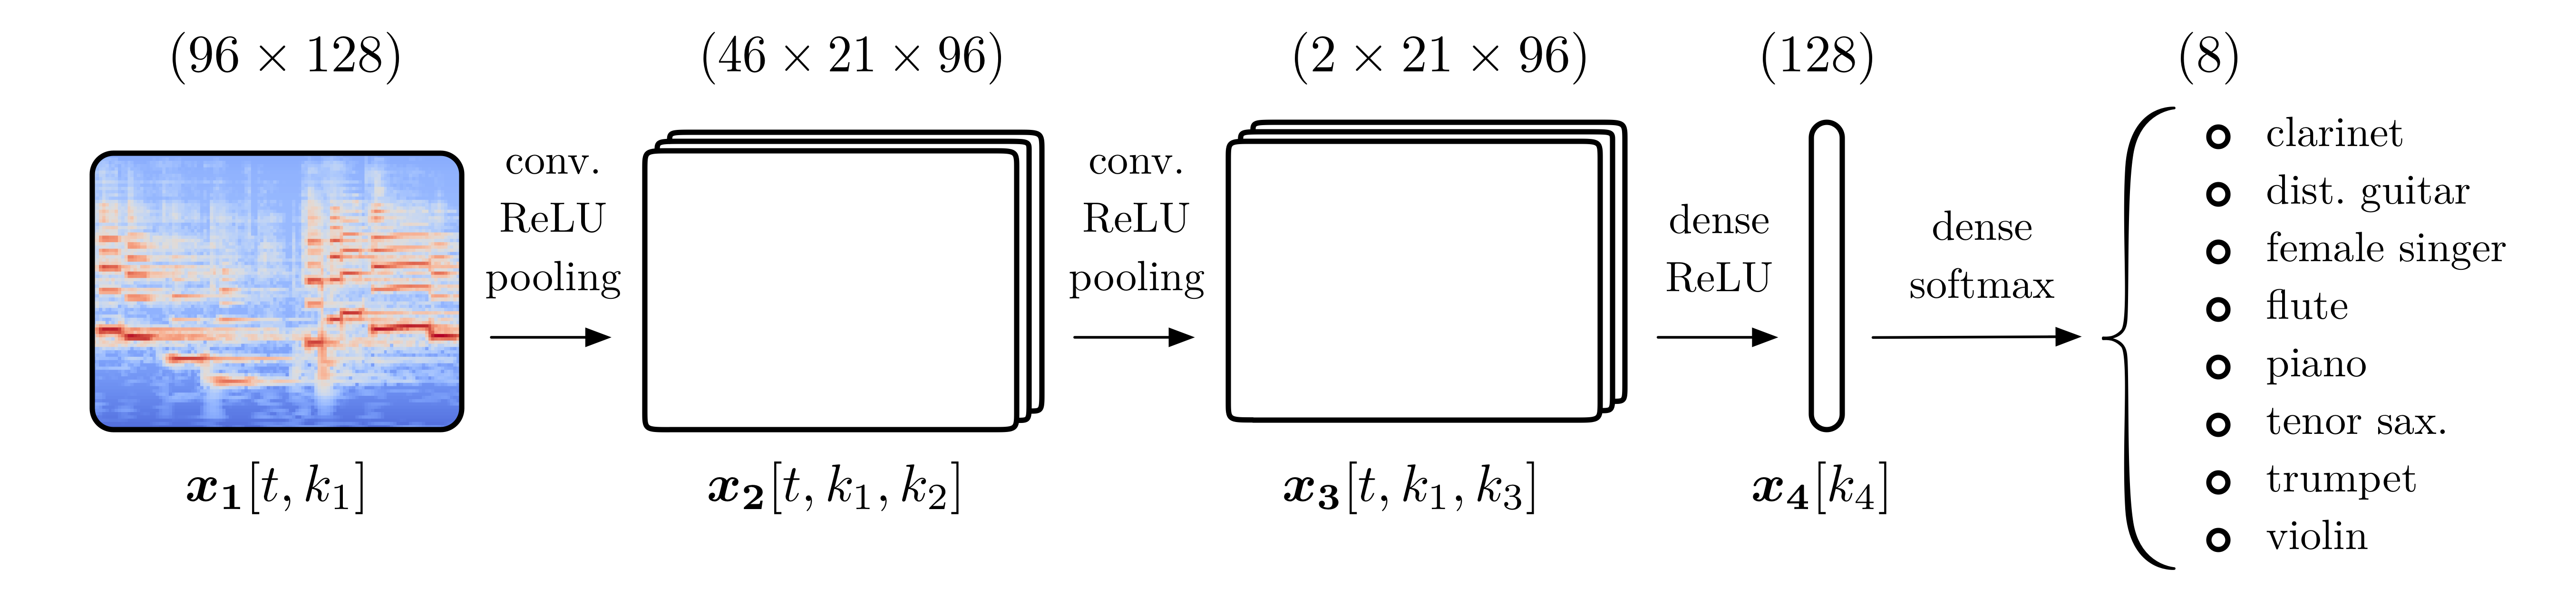
\includegraphics[width=17cm]{figs/architecture.png}}
        \end{picture}
    \end{center}
    \protect\caption{
Architecture of a convolutional network with full weight sharing. See text for details.
\label{fig:instrument-distribution}
}
\end{figure*}

We used the implementation from the librosa package \cite{McFee2015} with $Q=12$ filters per octave, center frequencies ranging from 55 Hz to 14 kHz (8 octaves from A1 to A9), and a hop size of 23 ms. Furthermore, we applied nonlinear perceptual weighting of loudness in order to reduce the dynamic range between the fundamental partial and its upper harmonics. A 3-second sound excerpt $\boldsymbol{x}[t]$ is represented by a time-frequency matrix $\boldsymbol{x_1}[t,k_1]$ of width $T=128$ samples and height $K_1=96$ MIDI indices, \ie 8 octaves.

Each layer in a convolutional network typically consists in the composition of three operations: two-dimensional convolutions, application of a pointwise nonlinearity, and subsampling.

First of all, we apply a family $\boldsymbol{W_2}[\tau,\kappa_1,k_2]$ of $K_2 = 32$ learned time-frequency convolutional operators, whose supports are constrained to have width $\Delta t$ and height $\Delta k_1$. Element-wise biases $\boldsymbol{b_2}[k_2]$ are added to the convolutions, resulting in the three-way tensor 
\begin{IEEEeqnarray}{rCl}
\IEEEeqnarraymulticol{3}{l}{
\boldsymbol{y_2}[t,k_1,k_2]} \nonumber \\
& = & \boldsymbol{b_2}[k_2] + 
\boldsymbol{W_2}[t, k_1, k_2] \overset{t,k_1}{\ast} \boldsymbol{x_1}[t, k_1]
\nonumber \\
& = &
\boldsymbol{b_2}[k_2] + 
\sum_{\substack{
0 \leq \tau < \Delta t \\
0 \leq \kappa_1 < \Delta k_1}}
\! \! \! \! \!
\boldsymbol{W_2}[\tau, \kappa_1, k_2]
\boldsymbol{x_1}[t-\tau, k_1-\kappa_1].
\IEEEeqnarraynumspace
\end{IEEEeqnarray}
The second step is the application of a pointwise nonlinearity. We have chosen the \emph{rectified linear unit} [ReLU] because of its popularity in computer vision and its computational efficiency.
 \begin{equation}
 \boldsymbol{y_{2}^{+}}[t,k_1,k_2] = \max \left( \boldsymbol{y_2}[t,k_1,k_2], 0\right)
 \end{equation}
 To achieve invariance to translation as well as frequency transposition, we pool neighboring units in
 the time-frequency domain $(t, k_1)$ over non-overlapping rectangles of width $\Delta t$ and height $\Delta k_1$.
\begin{equation}
\boldsymbol{x_2}[t,k_1,k_2] = \! \!
\max_{
\substack{
0 \leq \tau < \Delta t \\
0 \leq \kappa_1 < \Delta k_1}
} \! \!
\left\{
\boldsymbol{y_{2}^{+}}[t - \tau, k_1 - \kappa_1, k_2]
\right\}
\end{equation}
We apply a family $\boldsymbol{W_3}[\tau, \kappa_1, k_2, k_3]$ of $K_3$ convolutional operators that perform a linear combination of time-frequency feature maps in $\boldsymbol{x_2}$ along the channel variable $k_2$.
\begin{IEEEeqnarray}{rCl}
\IEEEeqnarraymulticol{3}{l}{
\boldsymbol{y_3}[t,k_1,k_3]} \nonumber \\
& = &
\sum_{k_2}
\boldsymbol{b_3}[k_2, k_3]
+ \boldsymbol{W_3}[t, k_1, k_2, k_3]
\overset{t,k_1}{\ast}
\boldsymbol{x_2}[t,k_1,k_2].
\IEEEeqnarraynumspace
\end{IEEEeqnarray}
After nonlinear rectification and max-pooling, the layer $\boldsymbol{y_3}$ turns into a non-negative tensor $\boldsymbol{x_3}[t,k_1,k_3]$.
\begin{equation}
\boldsymbol{y_4}[k_4] =
\sum_{t,k_1,k_3}
\boldsymbol{W_4}[t, k_1, k_3, k_4]
\boldsymbol{x_3}[t, k_1, k_3]
\end{equation}
We apply a ReLU to $\boldsymbol{y_4}$, yielding $\boldsymbol{x_4}[k_4] = \boldsymbol{y_4^{+}}[k_4]$. $\boldsymbol{y_5}[k_5] = \sum_{k_4} \boldsymbol{W_5}[k_4, k_5] \boldsymbol{x_4}[k_4]$.
\begin{equation}
\boldsymbol{x_5}[k_5] =
\frac{\exp \boldsymbol{y_5}[k_5]}
{  \sum_{\kappa_5} \exp \boldsymbol{y_5}[\kappa_5] }
\end{equation}
The above ensures that the coefficients of $\boldsymbol{x_5}$ are non-negative and sum to one, hence can be fit to a probability distribution.
\begin{equation}
\mathscr{L}(\boldsymbol{x_5}, \mathcal{I}) =
- \sum_{k_5 \in \mathcal{I}} \log \boldsymbol{x_5}[k_5]
+ \sum_{m=1}^{4} \lambda_m \Vert \boldsymbol{W_m} \Vert_2.
\end{equation}
The goal is to minimize the average loss $\mathscr{L}(\boldsymbol{x_5}, \mathcal{I})$ for across all pairs $(\boldsymbol{x}, \mathcal{I})$ in the training set.

% Random crops
% Categorical cross-entropy
The network is trained on categorical cross-entropy over shuffled mini-batches of size 512 with uniform class distribution. The learning rate policy for each scalar weight in the network is  \emph{Adam} \cite{Kingma2015}, a state-of-the-art online optimizer for gradient-based learning.

% Adam optimizer
% Shuffled examples with uniform class distribution
% Mini-batch learning
% Dropout

% Source-filter equation
% Ref to LeCun on disentangling factors of variability
% Ref to deeply supervised nets
% Ref to NIPS 2015
% Ref to Mallat 2016

% Different equation
% Comment extraneous vs joint
% Visualization to compare learned filters

\section{Limited weight sharing}
An Euclidean division of $k_1$ by $Q$ yields $k_1 = j_1 \times Q + \chi_1$.

\begin{IEEEeqnarray}{rCl}
\boldsymbol{y_2}[t,k_1,k_2]
= &
\boldsymbol{b_2}[j_1, k_2] & \nonumber \\
+ & 
\boldsymbol{W_2}[t, \chi_1, j_1, k_2] \overset{t,\chi_1}{\ast} \boldsymbol{x_1}[t, \chi_1, j_1].
\IEEEeqnarraynumspace
\end{IEEEeqnarray}

Limited weight sharing has been introduced by Abdel-Hamid et al. \cite{Abdel-Hamid2014}.

\section{Single-instrument classification}\label{sec:single-instrument}
\subsection{Experimental design}
In order to train the proposed algorithms, we used MedleyDB v1.1. \cite{Bittner2014}, a dataset of 122 multitracks annotated with instrument activations as well as melodic $f_0$ curves when present. We extracted the monophonic stems corresponding to a selection of eight pitched instruments [see Figure \ref{fig:instrument-distribution}]. Stems with leaking instruments in the background were discarded.
The evaluation set consists of 120 recordings of solo music collected by Joder et al. \cite{Joder2009}. We discarded recordings with extended instrumental techniques, since they are under-represented in MedleyDB.

\begin{table}
	\begin{center}
	\begin{tabular}{|c|cc|cc|}
		\hline
		& minutes & tracks & minutes & tracks \\
		\hline
		clarinet & 10 & 7 & 13 & 18 \\
		dist. guitar & 15 & 14 & 17 & 11 \\
		female singer & 10 & 11 & 19 & 12 \\
		flute & 7 & 5 & 53 & 29 \\
		piano & 58 & 28 & 44 & 15 \\
		tenor sax. & 3 & 3 & 6 & 5 \\
		trumpet & 4 & 6 & 7 & 27 \\
		violin & 51 & 14 & 49 & 22 \\
		\hline
		total & 158 & 88 & 208 & 139 \\
		\hline
	\end{tabular}
	\end{center}
	\caption{\label{table:single-label-durations}}
\end{table}

\subsection{Results}
Results are charted in Table \ref{table:single-label-results}.

\begin{table}
	\begin{center}
	\begin{tabular}{|l|c|}
		\hline
		Representation & Error rate (\%) \\
		\hline
		MFCC \& random forest & $-$ \\
		ConvNet, full weight sharing & $-$ \\
		ConvNet, limited weight sharing & $-$ \\
		\hline
	\end{tabular}
	\end{center}
	\caption{\label{table:single-label-results}}
\end{table}

\section{Polyphonic classification}\label{sec:polyphonic}
\subsection{Experimental design}

\subsection{Results}
Results are charted in Table \ref{table:multi-label-results}.

\begin{table}
	\begin{center}
	\begin{tabular}{|l|c|}
		\hline
		Representation & Error rate (\%) \\
		\hline
		MFCC \& random forest & $-$ \\
		ConvNet, full weight sharing & $-$ \\
		ConvNet, limited weight sharing & $-$ \\
		\hline
	\end{tabular}
	\end{center}
	\caption{\label{table:multi-label-results}}
\end{table}


\section{Conclusions}
Understanding the influence of pitch in audio streams is paramount to the design of an efficient system for automated classification, tagging, and similarity retrieval in music. 

% For bibtex users:
\bibliography{ISMIR2015template}

\end{document}
